\chapter{Project Execution}
\label{chap:execution}

A topic-specific chapter, of roughly $15$ pages
This chapter is intended to describe what you did: the goal is to explain the main activity or activities, of any type, which constituted your work during the project.

The content is highly topic-specific, but for many projects it will make sense to split the chapter into two sections:
 - one will discuss the design of something (e.g., some hardware or software, or an algorithm, or experiment), including any rationale or decisions made,
 - and the other will discuss how this design was realised via some form of implementation.

This is, of course, far from ideal for {\em many} project topics.  Some
situations which clearly require a different approach include:
\begin{itemize}
\item In a project where asymptotic analysis of some algorithm is the goal,
      there is no real ``design and implementation'' in a traditional sense
      even though the activity of analysis is clearly within the remit of
      this chapter.
\item In a project where analysis of some results is as major, or a more
      major goal than the implementation that produced them, it might be
      sensible to merge this chapter with the next one: the main activity
      is such that discussion of the results cannot be viewed separately.
\end{itemize}


Note that it is common to include evidence of ``best practice'' project management (e.g., use of version control, choice of programming language and so on).
Rather than simply a rote list, make sure any such content is useful and/or informative in some way: for example, if there was a decision to be made then explain the trade-offs and implications involved.



\section{Introduction}
The main activity of this project was the development of a mobile app that can usefully analyse climbers' technique and then provide them with various data whilst they trainig or climb for fun.

\subsection{User-Centered Iterative Design}
aims

iteration

spiral

testing

\section{Initial Survey}
To inform my first forays into the project, I released a simple quesstionaire online.
The questions can be found in Appendix~\ref{appx:1-ea} and my Ethics Application can be found in Appendix~\ref{appx:survey}.
I shared links to this survey across a variety of local climbing club pages, and got 49 responses in total. 
It must be mentioned that roughly half of these responses came in after I had already started development of the app, so although they did not all contribute to my initial development, I regularly checked the survey results and took into account any new opinions that were presented.
This is a benefit of an online survey, as I got a much wider reach, quantitity and range of responses compared to if I had performed a more traditional paper survey / interview at a climbing wall, with much less effort too.

\clearpage
\subsection{Survey Respondents}
\begin{wrapfigure}{r}{7.5cm}
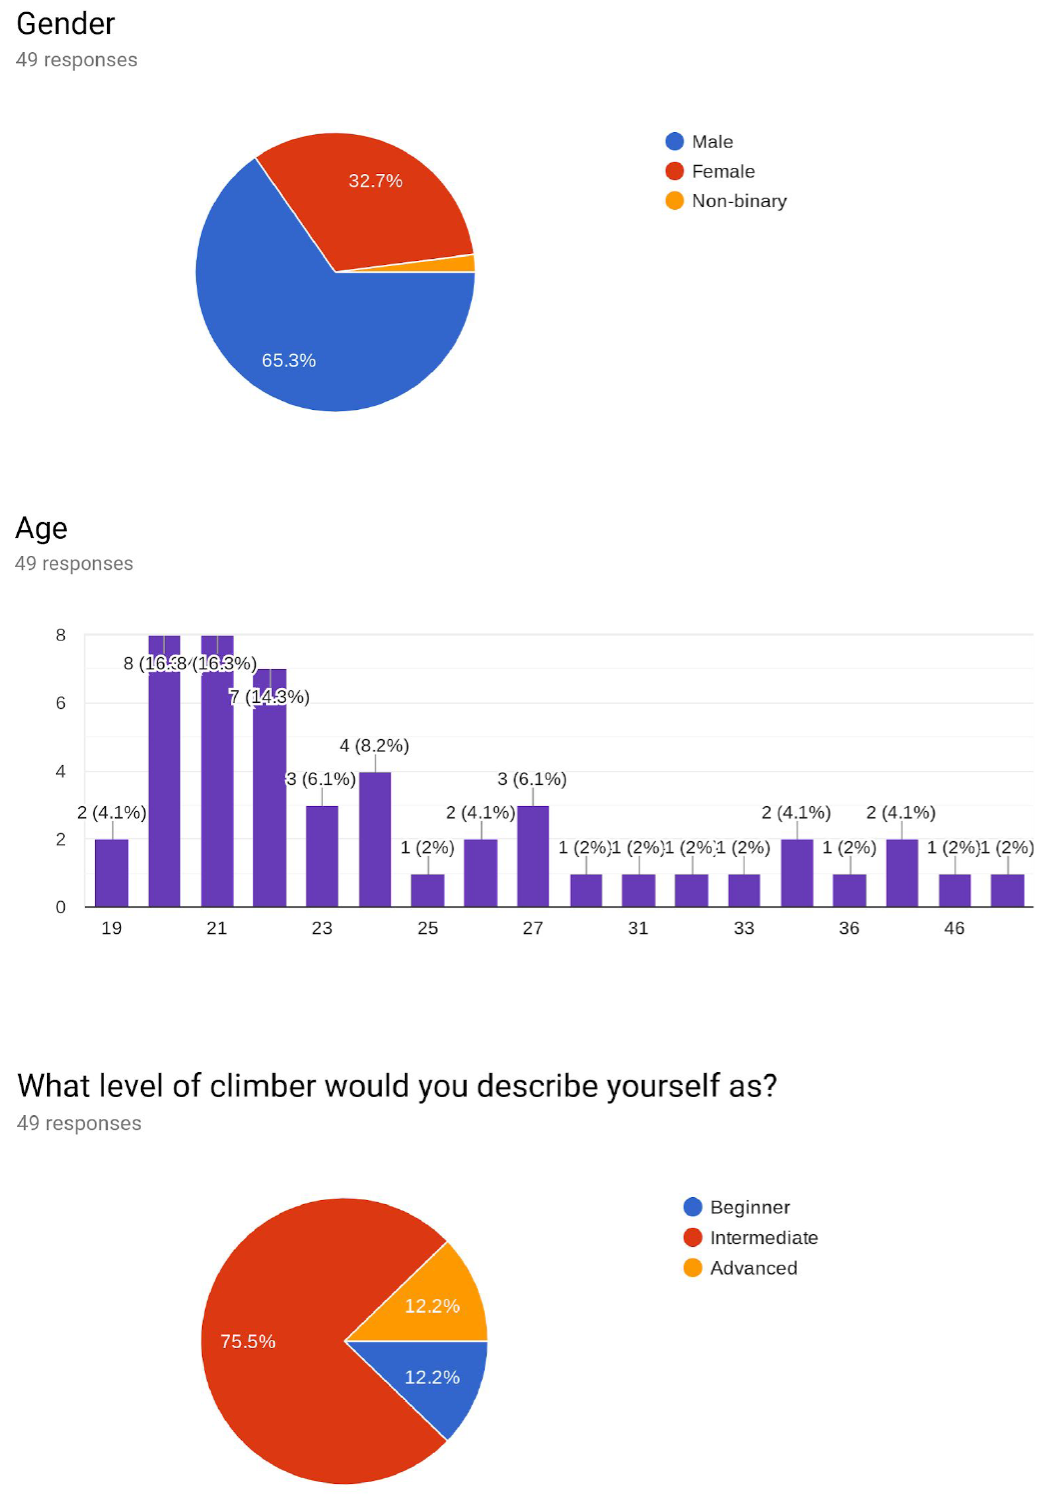
\includegraphics[width=7.5cm]{imgs/surveydemographics}
\caption{Demographics of Respondents to the Initial Survey}
\label{fig:surveydemographics}
\end{wrapfigure}
Some statistics on the demographics of the respondents can be seen in Figure~\ref{fig:surveydemographics}.
The male-female gender split is fairly consistent with the general indoor climbing population: 65\% male respondents compared to the 64\% stated in Rapelje's study on the demographics of climbers~\cite{climbing-sub-worlds}, and 65\% aged 19-24, compared to 60\% in that study.
This is because I made an effort spread the survey link across a range of local climbing pages and Facebook Groups, not just the student groups to get a more representative sample of views.

\subsection{Insights Gained From the Survey}
\subsubsection{Equipment Used}
To inform my decisions on what form my interactive device should take, I asked what items of equipment climbers often bring to the wall.
Everyone stated that they bring their own shoes, 90\% stated they bring a chalk-bag (a small hip-bag that contains powdered chalk for drying fingers and improving grip), and 31\% said they bring a small brush for cleaning dirty holds.
Only one respondent in this question included a phone in their list of equipment brought to the wall, and one even explicitly stated that they deliberately left their phone in their bag in order to "get away" from it. 

This provides a range of locations for locating a potential device, either inside the pocket of the chalk-bags, or attached to a brush, keeping with the light-weight aims of the project.

However, an app (and thus a phone) was the most discussed potential device for usage, with multiple suggestions that a "you would severely limit your possible audience by having the need for a device" as "everyone has a phone" so I should "stick with an app"

\subsubsection{Communication With Others Whilst Climbing}
Because an potential use of the device was to aid some of the common interactions that climbers had with friends at the wall, two of the questions in this initial survey asked what kind of things people wanted to hear whilst climbing, and what they often told their friends.

The most common response was "beta", which is a colloqial climbing term for advice on how body-positioning should be used to solve a tricky climb. 
<insert a definition?>
This can vary a lot between climbers, with each climb usually having two or more potential solutions.
Also, being able to "read" a climb to determine this beta is a tough and much-sought-after skill within the climbing community, to the extent that it is often nearly impossible for the very best in the sport, and thus definitely out of reach of any artificial Intelligence I could hope to create within this project.
An alternative, which was suggested by a few survey respondents, could have been to record (with either video or other sensors) a proficient climber climbing that route, and then showing that at a later date. 
However, this data-collection and -replay contradicted my initial aim of the device/app being able to be used anywhere - I wouldn't want to have to go around every few months and re-record somebody climbing every climb at each climbing wall just for the product to remain usable.

Another common interaction highlighted by the survey was "pointing out holds" to a climber, who is often so engrossed in the climb that they do not notice a certain location that they could put their hands or feet. This has an obvious potential use-case for a device, by using a colour video and existing computer-vision algorithms for coloured-blob-detection to find and then audio-relay the location of nearby holds to a climber.



\subsubsection{Requested Potential Features}
Arguably 


\section{Fundamental Early Decisions for Development}

\subsection{Platform Choice}
Despite researching a variety of different devices and form factors, one of the key aims of the project was always to make the final product as accessible as possible, therefore a OS-independent mobile app was decided upon.
By not using any extra equipment such as wristbands or 3d-cameras, the scope and ability of the final product could be limited - eg by lack of sensors and processing power - however limiting the need for anything but just a phone, which almost everyone owns, was a worthwhile sacrifice.
As well as making user-testing much easier, this choice also helped narrow the down the direction of the project, as working solely within the limits of what a mobile app could achieve meant that the capabilities of that platform could be fully stretched and explored.

The two inputs that mobiles can easily capture and that would potentially be most useful for the analysis of climbing technique were video recordings and accelerometer data.
Video recordings can be analysed with various computer vision techniques, and accelerometer data can be shown on a graph and analysed statistically for various outputs.


\subsection{Tool Selection}
\subsubsection{Development tool}
Next was to find a app-development tool that is quick and easy to use (for quick repeated iterations of the app), can easily import or link to the OpenCV Library (for the computer vision aspect), and is platform-independant (so any mobile phone owners can use the app, irrespective of OS).

Unity was chosen as it meets all three of those requirements, with a wide variety of Assets that can be imported.
Also having used the tool for games development in the past I was very familiar with using Unity, and knew that iterating over app designs would be quick and easy enough, compared to potentially wasting time learning how to use other tools when this one met all the requirements with the added benefit of previous experience using the tool.

\subsubsection{Version Control}
For version-control I used git, backed-up on GitHub.
Being a one-person project I rarely bothered with the overhead of using different branches, but the ability to roll-back to working code and releases, and to \verb|stash| and \stash|pop| various files at different times was very useful during development.
Once or twice a week, after a new feature or big set of fixes had been added, I would up-version the app, and release a compiled .apk binary to the project's GitHub page.
This allowed the easy re-installing of older versions when trying to locating a bug, as well as a clear documentation of all fixes and features included at each minor version upgrade.


\section{Initial Development}
The initial survey showed interest in computer-vision-aided video analysis of climbing, however I was wary of spending too much time trying to get it working.
Using previous recordings from my own climbing, the low-resolution images were noisy and not easy to detect much meaningful information, even when run slowly on a PC.
I knew that attempting to run intensive computer-vision algorithms on a mobile-phone processor in real-time would be even less effective, as well as draining battery very fast.

wizard of oz stuff with video body analysis
very tough complexity discussed in initial survey
usefulness of a app shouting out holds wasnt determined to be worth the time, although CV for this could be done in future.


Therefore the video-analysis was put on the back burner for a while, I kept chipping away at the problem, but focussed my main attention on the iterative developement of the actual app.

This required an app to use in the in-field studies, so I created a very simple app that could just record accelerometer data dn displayed the max and min.


smoothness

graph







Created accelerometer app
Saved to txt
Tested at redpoint - clicking start before stop overwrites (fixed)

Looked into time variation - also saved timestamp to csv, accelerometer data coming in varies in time, from 0.006s to 0.52s 
Especially issue when phone detected large acceleration, wanted to chane orientation, which slows down update.
Removed auto-orient,  moved to using fixedupdate and set timestep to 0.05 => 20 samples per second

12-13/3
Issue with precision of ticks being saved and parsed, couldnt use list of vectors, had to define struct to allow long,float types

V0.1 done - graphs visible
Dots had gaps - add lines - slow - remove dots ---  responsiveness research?

Seeing scale is good, so added axes label to let smaller graphs retain precision


Got second phone, looking into network possibilities
Unity networking - from games project known issues, plus requires a usable LAN, not easy with mobile at wall
Wifidirect?
Bluetooth?
Upload to cloud server?
 No unity support for any of them and all paid assets spenny.
Uploading to cloud would require scalability and some sort of user profile or something to differentiate and request the correct download, also slow/expensive for video? - nice sideeffect of backing up user profile to web, but then both devices signed in on same user?
Wifidirect has weird docs and unity had deprecated a lot of networking stuff, cant find info - look more?
Bluetooth seems simpler, nees a java code to be written then imported to unity as .jar plugin but possibility there.
What about utilising messaging? People could just send the file via social media apps?



14/3
For file transfer, and adding more info to climbing stuff such as associating video, a more reliable way of saving and loading climb data files was needed.
Also a general refactor from a codefile per screen to a seperate one for filehandling, data analytics, and graph rendering.
Moved to using unity serialise object as json instead of defining my own csv and writing my own parsers - better for future

In testnig climbers often would click on the scrollable graph viewer as if they were buttons, so i added the functionality to click and the view a larger graph of the climb, with a scroll bar.

Speed of graph drawing was slow, so added cached list of climbs in memory to save reading from disk every time 

Testing also said that putting phone in pocket annoying as records start of walking up to wall - added vibrating countdown timer

15/3
Also lack of pockets - got a chalkbag to put phone in for tests

Improved ui with answers to questions asked (what is recorded etc), and added cropping and deletion ability to climbview
Struggled with bluetooth stuff, required java code with exposed methods to link to unity c#
Used NativeShare asset which provides sharing on social media, turns out the bluetooth also works fine, job done, sharing works.
Started on file loading, used pragmas to select between unity editor (for testing) and android, used a liniked java class for android.
Added exception to filehandler to throw and display if file not unserialized correcetly

Issue: Cache invalidation issues with importing. Intialising anc updating cache on file load or file save? Which is import, it both loads and saves.
Infinite loop caused by self-initialising cache being updated by loader, which then causes the self-initialisation again. - selfinitialisaion checking for null, then reeiving full list, rather than asking for its list to be populated. Tied cache-updating to the saving of files instead of the loading of files.

Loads of issues with trying to open a file browser in android but working fully in windows - looked into SimpleFileBrowser asset













19/3
Diss meeting
Showed video scroller working
Redpoint climb to get data for poster demo - lining up video footage to acc data is tough
Set up timestamped-video filenames to help calculate offset


20/3 poster day went well


27/3
Set up automatic-viewing of accelerometer data, as was requested as an expected feature.
Also added variable back button as users expect to return to where they came from (ref?)

Many issues with video
Selecting a frame it doesn’t like on the webstream, then also codec / size issue with local file?
Limits to scaling on some videos = worst fking bug to replicate in thie system of time-matching and sending videos

Fixed the play before select frame by letting auto-play be switched off with hidden button under scrollbar, conveniently adds extra feature of letting video play by self, which was meaning to add

Go to frame still not working though on android
Fixed by playing a frame of video after skipping to frame, less responsive but more reliable. <- DESISION ON RELIABLITIY


V0.3 rc





Ok so videos recorded on the phone, either using native camera or using the in-app recorder, have codec issues
Somehow videos that are sent via whatsapp or telegram (and thus somehow transcoded) work fine, but obviously lose both the timestamped filename and creation metadata

So therefore the nice automatic matching of video data, with automatic guessing of the timestamp stuff, will have to be binned.
Instead an “add video” button on the view-climb page, with a manual “set video offset” thing, will have to happen.
Can’t think of a better way of matching up the recording, plus this will allow simply timing/syncing stuff in real life and then jus sending via whatever platform
Doesnt fix the non-playback issue though :(

Turning off multithreaded rendering makes video playback much smoother, but results in the frame not jumping to the selected one as easily, or at all, on slower android devices.


Added title editing and more analytics, as benig able to log grade and seeing more acceleration stuff was requested in survey

Put on play store

Added manual offset as the auto wasnt gonna work, not ideal but allows people to tweak it, can add auto as well if works in future


29/3
Re-enabled video recorder as testers thought everything in-app would be good (also can do instant video analysis-editing pre-share)

Instant share button for dual-device usage
Also testers said theyd expect to see it in gallery, and not lose the video straight after share/back button press, so used NativeGallery addon to save to gallery.

 Video playing works for landscape all along, no idea why portrait on ARM devices fails?
Readded simple offset calculation using parsed video name for cases whree file is recorded locally
Added more text and clearer button names for testing, sent off link to various people



1/4/19
Testers having issues with th epermissions stuff?




2/4 
Pete meeting, adding per-second smoothness to enable better linking to above numbers
added coloured boxed on graphdrawer to show dynamic seconds
remove autoredirect and added better page for after recording
Moved to using native gallery for video file browsing

3/4
Updated unity, permission blank screen fixed and videos all working



added axis labels after testing








































\section{Example Section}

This is an example section;
the following content is auto-generated dummy text.

\subsection{Example Sub-section}

\begin{figure}[t]
\centering
foo
\caption{This is an example figure.}
\label{fig}
\end{figure}

\begin{table}[t]
\centering
\begin{tabular}{|cc|c|}
\hline
foo      & bar      & baz      \\
\hline
$0     $ & $0     $ & $0     $ \\
$1     $ & $1     $ & $1     $ \\
$\vdots$ & $\vdots$ & $\vdots$ \\
$9     $ & $9     $ & $9     $ \\
\hline
\end{tabular}
\caption{This is an example table.}
\label{tab}
\end{table}

\begin{algorithm}[t]
\For{$i=0$ {\bf upto} $n$}{
  $t_i \leftarrow 0$\;
}
\caption{This is an example algorithm.}
\label{alg}
\end{algorithm}

\begin{lstlisting}[float={t},caption={This is an example listing.},label={lst},language=C]
for( i = 0; i < n; i++ ) {
  t[ i ] = 0;
}
\end{lstlisting}

This is an example sub-section;
the following content is auto-generated dummy text.
Notice the examples in Figure~\ref{fig}, Table~\ref{tab}, Algorithm~\ref{alg}
and Listing~\ref{lst}.

\subsubsection{Example Sub-sub-section}

This is an example sub-sub-section;
the following content is auto-generated dummy text.

\paragraph{Example paragraph.}

This is an example paragraph; note the trailing full-stop in the title,
which is intended to ensure it does not run into the text.
